\chapter{Introduction}
\label{chap:intro} % Always give a unique label
% use \chaptermark{}
% to alter or adjust the chapter heading in the running head

This chapter provides an introduction to this doctoral thesis. \Cref{sec:intro-motivation} motivates the research. \Cref{sec:problem-definition} defines the problem. \Cref{sec:intro-research-paradigm} gives an overview of the research methodology and defines the artifacts generated as outcome. \Cref{sec:data-collection} briefly discusses the datasets created and used in this thesis. \Cref{sec:intro-contributions} classifies the contributions of this thesis. \Cref{sec:intro-structure} provides an outlook of the structure, and \Cref{sec:intro-related-publications} lists the publications that have resulted from work on this thesis. 

\section{Motivation}
\label{sec:intro-motivation}

Software development is a process that involves creativity (\citealp{DBLP:journals/jss/AldaveVGM19,DBLP:journals/jss/DingsoyrNBM12}). Yet, practical software development projects are executed with specific requirements on time, budget and quality. In order to fulfill these requirements the development process must be monitored. For example, it is important to know what type of work is being done at a certain moment in time and by whom. This is for instance the case for large development projects where coordination mechanisms emerge spontaneously among developers who want to contribute with their code.
These type of projects are difficult to control for several reasons. First, there is no clear understanding in how far a certain piece of code advances the current status of the project. Second, a piece of code written by a developer goes through different stages of code-review and it is difficult to predict whether it will ever be merged with the main source. Third, coordination of work may involve a large number of message exchanges among many developers in forums. Hence, it is not feasible to manually oversee what work is going on at a particular point in time. 

Literature has tackled this problem from different angles. In the area of process mining approaches exist that exploit event logs for abstracting a process model \citep{Zerbino2021,vanZelst2021,DBLP:journals/tkde/AugustoCDRMMMS19,Rojas2016}. 
\todo[inline]{Example here}
In the area of software engineering, a major focus has been on the study of repositories in which the software is stored and worked on \citep{Farias2016,Matthies2020,Barros2021}. Contributions from this area provide several metrics that help with understanding various aspects of development. 
\todo[inline]{Example here}
However, process mining approaches only work with event logs where activities are explicitly recorded in the log. This is not the case with software development where data is rather unstructured. Likewise, software engineering approaches lack a perspective about work patterns. 


This study addresses the discovery of work patterns from software development event data. To this end, it defines concepts to capture work from software repositories. This allows to construct several discovery techniques that provide information about different perspectives of the development process. More specifically we categorize them into \emph{time}, \emph{case}, \emph{organizational} and \emph{control-flow}. The time perspective informs about temporal aspects of the process, such as when did an activity happen and for how long. The case perspective informs about characteristic of the different cases, such as the number of lines of code being produced at during the creation of each version of an artifact. The organizational perspective informs about the roles of the people in the context of the organization, such as developers, testers, etc. The control-flow perspective informs about the logical succession of activities, such as an artifact must first be implemented and then tested. 

In this sense, this work provides a bridge between process mining and software engineering. The findings of this work enable project managers as well as software developers to raise transparency about the actual development based on facts. As a result, it enables both understanding the current status and monitoring for potentially unwanted patterns of work.

%The rest of this proposal is organized as follows. \Cref{sec:problem-definition} describes the problem, the existing literature, and derives the solution requirements. \Cref{sec:state-of-field} provides background knowledge on the related fields of process mining, text mining, and mining software repositories. \Cref{sec:methods} explains the research method, the dataset and outlines the expected output of the thesis. \Cref{sec:preliminary-results} shows completed work so far. \Cref{sec:next-steps} outlines future steps towards the completion of this dissertation. \Cref{sec:dissertation-relevance} draws the implications for research and presents a dissemination plan.


\section{Problem Definition}
\label{sec:problem-definition}

%\todo[inline]{Here, too, include the four perspectives. Fig.1. can change: "4-perspectives of work" and include time, orga, control-flow, case. Include citations.}

%\todo[inline]{Check overlap of information provided here versus info provided in the background section. E.g. details of VCS.}

Software development processes are highly complex endeavours that require the coordination of multiple resources \citep{Kraut1995,Crowston2005}. Compared to standard business processes, they present the following characteristics. First, 
%although there is a planning phase, 
they involve creativity \citep{DeLaBarra2013,DBLP:journals/corr/abs-1305-6045,Aldave2019} when executing the tasks, i.e. there exists no strict process model that is followed by the developers to produce a new piece of code. Second, they are driven by methodologies \citep{Wynekoop1997}, e.g., \gls{rup}, Scrum\footnote{\url{https://www.scrum.org}}, Waterfall, etc. These methodologies constitute guidelines and best practices for project success. Third, they typically make use of software tools \citep{DBLP:books/daglib/0022944} such as \gls{its} \index{its}, \gls{vcs} \index{version control system} and \gls{ide} \index{integrated development environment}. Such tools typically record work activities into log files. Fourth, there is in general no process engine to control the execution \citep{Zahran1998}. Rather than that, a project manager or a Scrum master has to make sure that tasks are made available to the respective resources \citep{DBLP:books/daglib/001480}. Fifth, it is not trivial to obtain high level information on performance measures such as the burn-down rate, which are resource bottlenecks, what are time requirements for certain tasks, what type of work is actually being done, and how productive are people working in certain tasks, etc \citep{DBLP:journals/csur/MeidanGRE18}. Hence, there is the need for algorithms and tools that help extracting this knowledge.

\begin{figure}
	\centering
	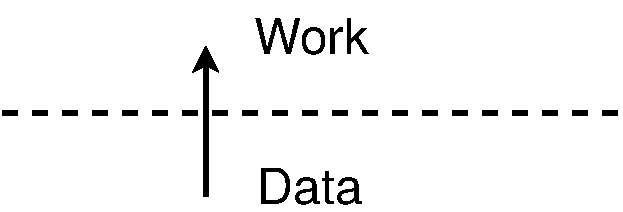
\includegraphics[width=0.4\linewidth]{figures/data-to-work}
	\caption{Automatically derive work from trace data}
	\label{fig:data-to-work}
\end{figure}


Software development processes fall into the category of \emph{project-oriented business processes} \citep{DBLP:conf/bpm/BalaCMRP15}. 
That is, they are rather ad-hoc plans performed with limited resources and time, but with a clear goal: develop a software artifact. Unlike classic business processes which are best captured with notations such as Petri nets and \gls{bpmn}, software development processes are more akin to one-time plans, which are usually captured by models such as Gantt and PERT diagrams. The following example captures the essence of a typical software development process in practice, such as for instance in Google LLC \citep{Henderson2017}.


\begin{quote}
	A new software version or feature needs to be developed. Unquestionably, Google has know-how on software development. However, before starting the implementation phase, precise requirements for tasks must be formulated. These tasks are stored in \gls{its} and referred to as \emph{issues}. Usually effort estimation values are assigned to each of them. Subsequently time and resources are allocated to the tasks. This starts the implementation phase. During this phase, resources work on tasks in a creative way, choosing among available tasks according to their own skills and expertise. In order to save the progress, developers issue a so-called \emph{commit} command which creates a new version of the modified files on the \gls{vcs}. Likewise, every time a certain task (which may be carried out through by different commits) is completed, the corresponding issue is marked as done. Both commits and issues can be commented by the users, respectively to document the changes and raise a discussion for increasing understanding the problem.
\end{quote}

Several tools are used by software project participants to support their work. Therefore, traces about the overall process are typically available in different repositories and artifacts, e.g., spreadsheets, word processor documents, programming languages files, emails, etc. This makes it cumbersome to obtain knowledge about the overall business process through manual inspection. Also, it is a challenge to automatically \emph{extract} work information from unstructured data such as user comments when working on tasks. For instance, existing solutions (e.g., process mining algorithms) are not able to provide informative results when the data is not available as a structured single event log where activities are explicitly labeled. Likewise, other software tools (e.g. GitHub) limit themselves at providing only process-unaware statistical information (e.g., number of commits in a file).

%Therefore, the overall challenge is to understand which are important events that track development work in the repository. 


While obtaining an overarching view on software development is challenging, there are still repositories that can be exploited to obtain process knowledge. One tool that provides important traces of the development work is \gls{vcs}. This tool is used to keep track of the different versions of files created by users and to manage their collaboration. Not only supports it keeping track of file versions, but also allows users to associate a textual comment that describe the changes made. Therefore, a new version of a particular file is created as the result of an activity done by a user. The evolution of these versions, along with information about the users and their comments can be retrieved from these type of tools in the form of semi-structured event logs. It is then a challenge how to discover the business process from events (e.g., lines of code changed, comments, user information) present in these logs.

%
%\todo{JM: I think you have to develop much more clearly how it is difficult to extract certain pieces of information from version control systems.} 

%An important dimension of the software development process is the work dimension, i.e. the process. This perspective is particularly interesting to project managers. One of their goal is to know whether the planning phase was realistic with respect to the development efforts. Existing software repositories allow for many ways to access their log files. These log files offer factual information about actions done by the process participants to change the repository state.

\begin{figure}[h]
	\centering
	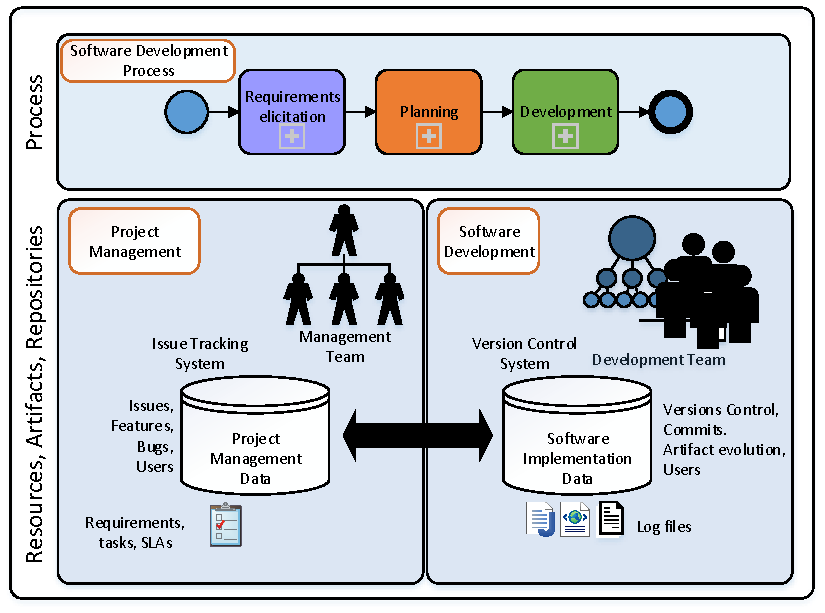
\includegraphics[width=\linewidth]{figures/big-picture}
	\caption{Software development scenario with two repositories used for project management and software development, respectively.}
	\label{fig:big-picture-sd}
\end{figure}

\Cref{fig:big-picture-sd} illustrates such problem scenario. Software development relies on tools like \gls{its} (e.g., JIRA, GitHub Issues) and \gls{vcs} (e.g. Subversion, Git). \Gls{its} is used for tracking the project management aspect. This aspect offers plan related information, such as issues, features, bugs, text, planned and executed tasks, timestamps, stories, and effort estimation (e.g., story points in JIRA).
\Gls{vcs} offers information about work traces, such as versions of the artifacts, number and content of commits done by developers, artifacts evolution, users and their comments, and timestamps of each action. 
% Please add the following required packages to your document preamble:
% \usepackage{booktabs}

% \usepackage[normalem]{ulem}
% \useunder{\uline}{\ul}{}
%\vspace*{-.5cm}
\newcommand{\rowsep}{\vspace*{2pt}}
%\newcommand{\colsep}{\hspace*{52pt}}
\begin{table}[h]
%	\small
	\caption{An excerpt of a VCS log data}
	\label{tab:vcs-log-data1}
	\setlength{\tabcolsep}{6pt}
%	\setlength\belowcaptionskip{-20pt}
\centering
%\resizebox{.99\textwidth}{!}{%
%\begin{tabular}{@{ }cm{.7cm}m{2cm}m{4.8cm}m{7cm}@{ }}
\begin{tabular}{@{~~}lm{1cm}m{1.4cm}m{1.7cm}m{5cm}@{~~}}
\toprule
\textbf{Id} & \textbf{Resource} & \textbf{Date}                          & \textbf{Comment}                          & \textbf{Diff}                                                                                                                                                                                                                                                                                   \\ \midrule 
%\rowcolor{lightgray}
1          & John    & 2017-01-31 12:16:30 & Create readme file                   & \begin{tabular}[c]{@{}l@{}}diff --git a/README.md b/README.md\\ @@ -0,0 +1 @@\\+\# StoryMiningSoftwareRepositories \end{tabular}                                                                                                                                                          \\ \rowcolor{lightgray}
\addlinespace
2          & Mary    & 2017-02-01 10:13:51 & Add a license                   &  \begin{tabular}[c]{@{}l@{}}diff --git a/README b/README\\ @@ -1,0 +2,3 @@\\ +The MIT License (MIT)\\ +\\ +Copyright (c) 2015 Mary+\end{tabular}                                                                                                                                     \\ \addlinespace
%\rowcolor{lightgray} 
3          & Paul    & 2017-02-02 16:10:22 & Updated the requirements.               &  \begin{tabular}[c]{@{}l@{}}diff --git a/README.md b/README.md\\ @@ -1,4 +1,5 @@ \\ + \# string 1, string 2, string 3\\ \\ diff --git a/requirements.txt b/requirements.txt\\ @@ -0,0 +1 @@\\ +The software must solve the problems\end{tabular} \\ \rowcolor{lightgray} \addlinespace

4          & Paul    & 2017-02-02 15:00:02 & Implement new requirements &  \begin{tabular}[c]{@{}l@{}}diff --git a/model.java b/model.java\\ @@ -1,9 +1,10 @@ \\ {+public static methodA()\{int newVal=0;}\\ @@ -21,10 +23,11 @@\\ + "1/0",,"0/0",\\ \\ diff --git a/test.java b/test.java\\ @@ -0,0 +1,2 @@\\ +//test method A\\ +testMethodA()\end{tabular}  \\ \bottomrule
\end{tabular}%
%}
\end{table} 


Although different technologies exist in practice (e.g., Subversion, Mercurial, Git), the information contained in the logs can be roughly summarized by \Cref{tab:vcs-log-data1}. \todo{Maybe I can change this table with a more generic one that contains all information?}  The table displays an excerpt of a \gls{vcs} log, i.e., a set of user commits, after having extracted and structured the data according to five attributes. The semantics of the  attributes is a follows: 
\begin{inparaenum}[\itshape i)]
	\item \emph{Id} is a unique identifier;
	\item \emph{Resource} is the resource that issued the commit;
	\item \emph{Date} is a timestamp associated to the time and date the commit was stored in the system;
	\item \emph{Comment} is a user comment on the changes made;
	\item \emph{Diff} is low-level information on the difference between the current and the previous version, for each file.
\end{inparaenum} 
Likewise, information about issues from \gls{its} can be extracted and presented in a tabular way. In this case, other attributes are more important. These attributes can be, for example, the status of issues and the conversations that take place around them. %As the relation between \gls{its} and \gls{vcs} about requirements-implementation, we can narrow down our research question to the following. \emph{\textbf{RQ:} How does the specification of user stories influence software development work?} 
%In the more specific case, \gls{vcs} logs consist of an ordered set of \emph{commits} bearing information about users, files, timestamp, comments and type of change that were stored at particular moment in time. \Gls{its} typically come with richer information, most importantly they inform about users, task, type of task (e.g., bug, new feature, requirement, etc), timestamps, related issues, etc. 
%Many types of analyses can be performed on such feature rich data once they have been properly correlated and structured. 
Hence, studying the co-evolution of these two repositories can help extracting relevant knowledge about the software development process. 

More precisely this work seeks answer to the following research question. \textbf{RQ}: \emph{How can we make use of project event data to gather insights about the software development process that are informative to managers?} 
Because the project managers can benefit from a process view to better analyze hidden aspects of the software development process, this work takes a process mining stance on the problem. Therefore, the main research question is broken down into the following four subquestions. Each of them addresses \textbf{RQ} with respect to the four perspectives of a process that are useful to discover the event data \citep{DBLP:books/sp/Aalst16}.

%In the light of the above considerations, we derive the following requirements for extending process mining towards the analysis of software repositories.
%Owing to \gls{pm} literature, the research question (\textbf{RQ}) can be further broken down to the four process mining perspectives. 
%From here, we derive the four fundamental requirements that satisfy \gls{msd}.

\begin{inparadesc}
	\item[RQ1.] \emph{How can we use project event data to extract information about the \textbf{temporal} perspective of activities?} 
	%	For example, an answer to this question would look like: the development activity has a duration of 2 weeks on average, the average time of task creation is 15 minutes, etc. 
	
	\item[RQ2.] \emph{How can we use project event data to extract information about the \textbf{case} perspective?} 
	%	For example, an answer to this question would look like: all the bugs are solved in a 3 steps iteration, or a quality piece of code takes a conversation with 3 people and is successfully merged into the main branch after 1 week, etc.
	
	\item[RQ3.] \emph{How can we use project event data to extract information about the \textbf{organizational} perspective?} 
	%	For example, an answer to this question would look like: the software development is carried out by a team of 4 people, the actual user roles in the company are developer and tester, etc.
	
	\item[RQ4.] \emph{How can we use project event data to extract information about the \textbf{control-flow} perspective?} 
	%	For example, an answer to this question would look like: the testing is always done before development, or while new features are worked on, also new requirements are created, etc. Note that, differently from \textbf{RQ1} this question focuses on the logical connection and order of activities.
	
\end{inparadesc}

\section{Research Methodology and Generated Artifacts}
\label{sec:intro-research-paradigm}

%\todo[inline]{Here goes Peffers \citep{Peffers2008}
%	
%	Make clear what type of contribution you are proposing. E.g., engineering: set of techniques, algorithms, etc.
%	
%	This section presents the research method. It also describes the dataset and outlines the expected research outcome.
%}

This thesis is positioned as design science \citep{Hevner2004}.
Information systems research is an interdisciplinary field of study that uses theories from social sciences, economics, and computer science. The field can be divided into two complementary paradigms: \emph{behavioral science} and \emph{design science}. Behavioral science aims at developing and justifying theories in order to explain or predict information systems phenomena \cite[]{Gregor2006}. Design science focuses on the creation and evaluation of innovative design \emph{artifacts} \cite[]{Hevner2004}. \Cref{fig:DS-process} illustrates the design science approach as a process \citep{Peffers2008}. 

\begin{figure}[h]
	\centering
	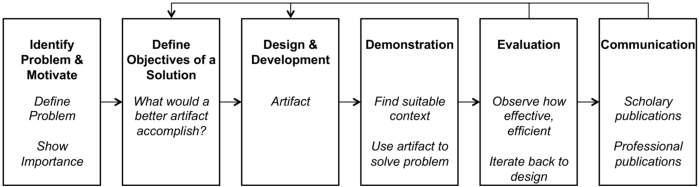
\includegraphics[width=\linewidth]{figures/DS-process}
	\caption[The Design Science Research process]{The Design Science Research process, adapted from \citep{Peffers2008}}
	\label{fig:DS-process}
\end{figure}

%This doctoral thesis employs both design and behavioral science. Following the approach suggested by \cite[]{Berente2018}, real life data will be used for data-driven computationally-intensive theory development. \todoinline{JM: You really want to develop theory, or you aim to provide techniques? I think you work is more about providing technique - that are useful to inform the mentioned approach to theory building.} This approach can be seen as a combination between behavioral science and design science. The behavioral perspective is given by traditional theory development based on manual coding, e.g. \gls{gtm}. The design perspective is given by the creation of novel artifacts (e.g., software algorithms) that use trace data to automatically discover theory, e.g, \gls{ctd}. This thesis uses real world data gathered from the SHAPE project\footnote{\url{https://aic.ai.wu.ac.at/shape-project/}} and \gls{oss}. This data will be used both for generating propositions about process aspects and developing novel artifacts. These artifacts apply process mining methods to a new domain, also referred to as exaptation \citep{Gregor2013}. 

%With reference to \gls{dsr} process in \Cref{fig:DS-process}, next sections show the design and development of the dataset and artifacts for addressing the requirements posed in \Cref{sec:problem-definition}.
%
%
%The following subsections explain the research method adopted in relation to \gls{dsr}. 

This thesis develops four artifacts \textbf{A1}, \textbf{A2}, \textbf{A3}, \textbf{A4} respectively addressing the four research questions \textbf{RQ1}, \textbf{RQ2}, \textbf{RQ3}, \textbf{RQ4}. Each artifact is devised following the \gls{dsr} approach \citep{Peffers2008}. These artifacts are interconnected to one another in that each of them tackles a different perspective of the overarching software development process. Their combinations enables a view on the \emph{real} Gantt chart of the project, as illustrated in \Cref{fig:big-solution}. Such techniques are also useful to inform computationally-driven theory building~\citep{DBLP:journals/isr/BerenteSS19}.

\begin{figure}[]
	\centering
	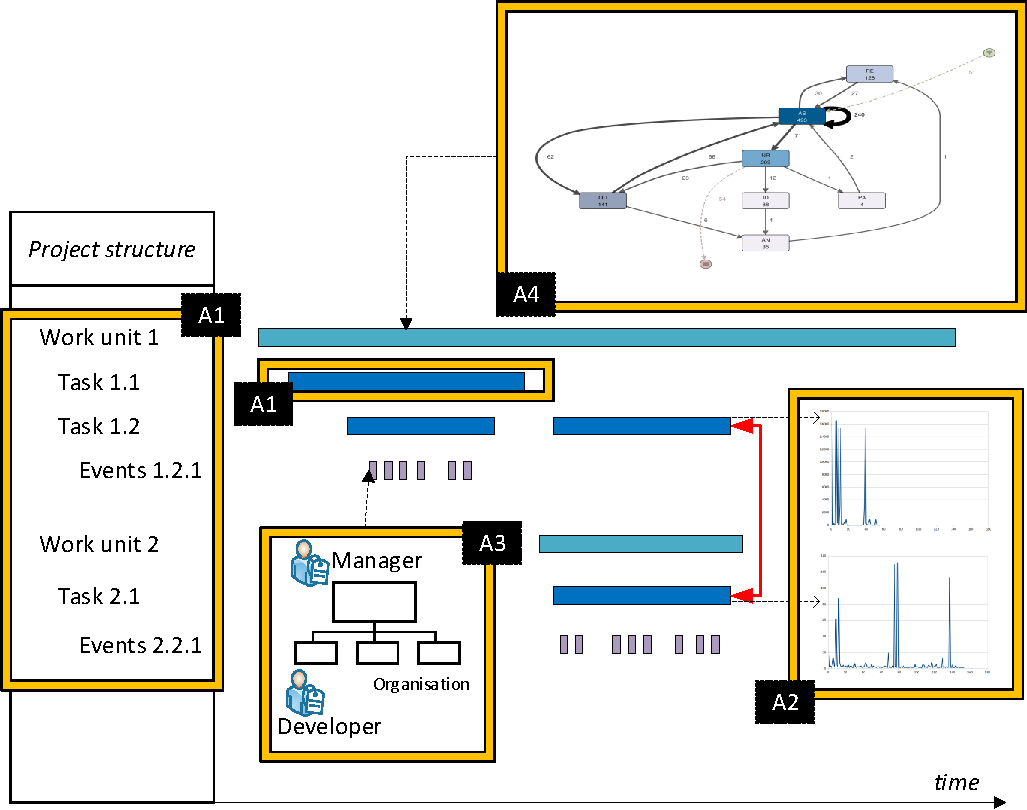
\includegraphics[width=\linewidth]{figures/big-solution2-crop.pdf}
	\caption{The empirical Gantt chart of software development. The four process perspectives combined.}
	\label{fig:big-solution}
\end{figure}

Research rigor and validity are ensured by evaluating the artifacts with the \gls{feds} \citep{Venable2016}. \Gls{feds} provides strategies for evaluating \gls{dsr} artifacts. More specifically, it takes into account two dimensions
\begin{inparaenum}[\itshape i)]
	\item the functional purpose of the
	evaluation (formative or summative); and 
	\item the paradigm of the evaluation (artificial or naturalistic).
\end{inparaenum} 
Moreover, it provides four steps for chinfinicaoosing an appropriate evaluation strategy
\begin{inparaenum}[\itshape i)]
	\item explicate the goals of the evaluation;
	\item choose the evaluation strategy or strategies
	\item determine the properties to evaluate; and
	\item design the individual evaluation episode(s). 
\end{inparaenum} In the following, we describe each designed artifact and their evaluation. 

\cite{Gregor2020} define a schema for defining \emph{design principles} so that they are understandable and useful in real world context. \todo{Shoud I define design principles according to their schema? This may be a good idea!}




%% Please add the following required packages to your document preamble:
% \usepackage{booktabs}
% \usepackage[normalem]{ulem}
% \useunder{\uline}{\ul}{}
% \usepackage{longtable}
% Note: It may be necessary to compile the document several times to get a multi-page table to line up properly
\begin{longtable}[c]{@{}p{1.2cm}p{2.5cm}p{5cm}p{3cm}p{4cm}@{}}
\toprule
\textbf{Artifact} & \textbf{Features}                              & \textbf{Goals}                                                                                                                                                                                                                                                           & \textbf{Evaluation}                                                                                                                                  & \textbf{Iteration episodes}                                                                                                   \\* \midrule
\endhead
%
\bottomrule
\endfoot
%
\endlastfoot
%
\textbf{A1}       & time information                               & General goal: has to be applicable, usable, simple and provide overview as well as detailed view                                                                                                                                                                         & Quick and simple: the technique is directly evaluated with real data                                                                                 & First iteration (formative): initial design of gantt chart                                                                    \\
                  & duration of activities                         & Rigor: assured by the design science approach                                                                                                                                                                                                                            &                                                                                                                                                      & Second iteration: evaluation of successful identification of events and project structure                                     \\
                  & structure of the project                       & Uncertainty and risk reduction: artifacts is technically infeasible, data is unavailable                                                                                                                                                                                 &                                                                                                                                                      & Third iteration: run of the tool on real projects and provide a visualization                                                 \\
                  & granularity of events                          & Ethics: “big-brother is watching you” effect on people                                                                                                                                                                                                                   &                                                                                                                                                      &                                                                                                                               \\
                  &                                                & Efficiency: find all time patterns, algorithm runs in a reasonably short time                                                                                                                                                                                            &                                                                                                                                                      &                                                                                                                               \\* \midrule
\textbf{A2}       & difference between different instances of work & General goal: has to be applicable, usable, simple and provide overview as well as detailed view                                                                                                                                                                         & Quick and simple: the technique is firstly evaluated with a toy example, then revised and applied to a large number of software development projects & First iteration (formative): initial design of artifact and results  visualizations                                           \\
                  & amount of changes                              & Rigor: assured by the iterations                                                                                                                                                                                                                                         &                                                                                                                                                      & Second iteration: revision and choice of final visualization                                                                  \\
                  & handle unstructured data from comments         & Uncertainty and risk reduction: artifacts is technically infeasible adressed by developing by smaller iterations, data is unavailable addresses by local copy, results interpretation is hard addressed by mining processes from text                                    &                                                                                                                                                      & Third iteration: evaluation of efficacy on retrieving features                                                                \\
                  & evolutionary analysis of changes               & Ethics: n/a because data is public                                                                                                                                                                                                                                       &                                                                                                                                                      & Fourth iteration: run the technique on toy exampe (artificial evaluation). Validate efficacy and usefulness. Revise artifact. \\
                  & uncover work dependencies                      & Efficiency: find all work dependencies in a reasonable time                                                                                                                                                                                                              &                                                                                                                                                      & Firfth iteration: run the technique on real data sets from GitHub projects (naturalistic evaluation)                          \\* \midrule
\textbf{A3}       & determine roles of users                       & General goal: has to aplicable and provide correct classification of roles                                                                                                                                                                                               & Quick and simple: the technique is evaluated with real data from industry partners                                                                   & First iteration (formative): initial design of simple artifact voted to a simple and structured represenation of the data     \\
                  & handle user comments                           & Rigor: assured by the iterations                                                                                                                                                                                                                                         &                                                                                                                                                      & Second iteration: selection of features and classifiers traininig. Selection of the best features and classifiers.            \\
                  & automatically classify resources               & Uncertainty and risk reduction: risk is that artifact incorrectly classifies reources, this is reduced by using different training sets from industry partners and otaining feedback                                                                                     &                                                                                                                                                      & Third iteration: evaluation of results with real data from partners and feeback                                               \\
                  &                                                & Ethics: there is a risk of obtaining information about people’s work. This is mitigated by NDA signed by the parties involved                                                                                                                                            &                                                                                                                                                      &                                                                                                                               \\
                  &                                                & Efficiency: evaluated in terms of precision and recall                                                                                                                                                                                                                   &                                                                                                                                                      &                                                                                                                               \\* \midrule
\textbf{A4}       & handle comments from forum conversations       & General goal: has to aplicable to pull requests and provide informative and reliable process models about the generation of an idea                                                                                                                                      & Technical risk and efficacy: the technique is firstly evaluated with an initial dataset, then revised and evaluated with other projects              & First iteration (formative): initial exploratory analysis on the applicability of process mining techniques on pull requests  \\
                  & discover a process model                       & Rigor: assured by the iterations                                                                                                                                                                                                                                         &                                                                                                                                                      & Second iteration: evaluation of process mining methods and assessment of statistical significance of results                  \\
                  &                                                & Uncertainty and risk reduction: risks are: 1) activities of business processes are not mapped correctly – mitigated by manual annotation 2) the resulting model is not informative – mitigated by statistical techniques voted to cluster traces into significant groups &                                                                                                                                                      & Third iteration: mine process models that are statistically significant and analyze the idea generation patterns              \\
                  &                                                & Ethics: n/a. Only data from open source repositories will be used                                                                                                                                                                                                        &                                                                                                                                                      &                                                                                                                               \\
                  &                                                & Efficiency: the artifact can deal with complex projects quickly                                                                                                                                                                                                          &                                                                                                                                                      &                                                                                                                               \\* \bottomrule
\end{longtable}

\subsection{Discovering the Temporal Perspective of the Software Development Process (Artifact A1)} 
%~\\\noindent\rule[1ex]{2.5cm}{2pt}~\\	
Design objectives of \textbf{A1} aure \begin{iiilist}
	\item has to be applicable, 
	\item usable, 
	\item simple and,
	\item provide overview as well as detailed view.
\end{iiilist} 
The following features are included: 
\begin{iiilist}
	\item time information,
	\item duration of activities,
	\item structure of the project, and
	\item roll-up and drill-down on granularity of events.
\end{iiilist}
Evaluation goals are 
\begin{iiilist}
	\item rigor,
	\item uncertainty and risk reduction,
	\item ethics, and
	\item efficiency.
\end{iiilist}
They are respectively addressed as follows. Rigor is assured by the design science approach. Uncertainty involves technical infeasibility and unavailuability of the data. Infeasibility risk is reduced by starting from the design of small artifacts with basic features and incrementally improve. Unavailability risk is reduced by replication of the dataset locally. An ethics problem may regard the “big-brother is watching you” effect on people. This will be solved considering only data from partners and public repositories. Efficiency is evaluated by measuring whether all time patterns are found in a reasonably short time.

This artifact is evaluated through a Quick \& Simple strategy \citep{Venable2016}, i.e., the technique is directly evaluated with real data. This will include three iteration episodes 
\begin{iiilist}
	\item initial design of Gantt chart (formative)
	\item evaluation of successful identification events, their duration and project structure; and 
	\item run of the tool on real projects and provide a visualization (summative).
\end{iiilist}



\subsection{Discovering the Case Perspective of the Software Development Process (Artifact A2)} 
%Addresses RQ2.
%~\\\noindent\rule[1ex]{2.5cm}{2pt}	
Design objectives of \textbf{A2} include applicability, simplicity and providing comparison of different cases. The following features are designed: 
\begin{iiilist}
	\item difference between work instances;
	\item measure of work: amount of changes;
	\item handle unstructured data from comments;
	\item evolutionary analysis of files; and
	\item uncover work dependencies.
\end{iiilist}
Evaluation goals are as follows. Rigor is assured by the iterations. Uncertainty and risk reduction consist in: technical infeasibility -- addressed through development by smaller iterations, data unavailability -- addressed by local replication of data, and simplicity of results -- addressed by exploiting user comments and derive informative process labels. Ethics problems do not arise as the data for this artifact is already public on GitHub. Efficiency is evaluated by finding all work dependencies in a reasonable time. 

This artifact is evaluated through a Technical risk \& Efficacy strategy (see \cite{Venable2016}), i.e., the technique is firstly evaluated with a toy example, then revised and applied to a large number of software development projects. Five iteration episodes are included: 
\begin{iiilist}
	\item initial design of artifact and results  visualizations(formative);
	\item revision and choice of final visualization;
	\item evaluation of efficacy on retrieving features;
	\item run the technique on toy example (artificial evaluation), validate efficacy and usefulness, revise artifact; and
	\item run the technique on real data sets from GitHub projects (summative and naturalistic evaluation).
\end{iiilist}



\subsection{Discovering the Organizational Perspective of the Software Development Process (Artifact A3)}
%~\\\noindent\rule[1ex]{2.5cm}{2pt}
Design objectives of \textbf{A3} include applicability and correct classification of roles. The following features are designed 
\begin{iiilist}
	\item determine roles of users;
	\item handle user comments; and
	\item automatically classify resources.
\end{iiilist}
Evaluation goals are as follows. Rigor is assured by the iterations. Uncertainty and risk reduction regard classification. Incorrect resource classification risk is reduced by using different training set data from industry partners and obtaining feedback. An ethics risk is about obtaining information about people's work. This is mitigated by NDAs signed by the parties involved. Efficiency is evaluated in terms of precision and recall. 

This artifact is evaluated through a Quick \& Simple strategy (\cite{Venable2016}), i.e., the technique is evaluated with real data from industry partners. Three iteration episodes are included: 
\begin{iiilist}
	\item initial design of the artifact voted to a simple and structured representation of the data (formative)
	\item exploration and selection of the best features and classifiers.
	\item evaluation of results with real data from partners and feedback (summative + naturalistic).
\end{iiilist}

\subsection{Discovering the Control-Flow Perspective of the Software Development Process (Artifact A4)} 
%Addresses RQ2.
%\rule{3cm}{1pt}
%~\\\noindent\rule[1ex]{2.5cm}{2pt}
Design objectives of \textbf{A4} are its applicability to pull requests and its functionality to provide informative and reliable process models about specific work patterns. The following features are designed.
\begin{iiilist}
	\item handle comments from forum conversations, and
	\item discover a process model.
\end{iiilist}
Evaluation goals are considered as follows. Rigor is assured by the iterations. Uncertainty and risk reduction the following
\begin{iiilist}
	\item activities of business processes are not mapped correctly -- mitigated by manual annotation; and
	\item the resulting model is not informative -- mitigated by statistical techniques voted to cluster traces into significant groups.
\end{iiilist} Ethics problems do not arise because only data from open source repositories will be used. Efficiency is measured by the extent to which the artifact can deal with complex projects quickly.

This artifact is evaluated through a Technical risk \& Efficacy strategy (see \cite{Venable2016}), i.e., the technique is firstly evaluated with an initial well-known dataset, then revised and evaluated with other projects. Three iteration episodes are included: 
\begin{iiilist}
	\item initial exploratory analysis on the applicability of \gls{pm} techniques on pull requests (formative);
	\item evaluation of \gls{pm} methods and assessment of statistical significance of results; and
	\item mine process models that are statistically significant and analyze the idea generation patterns (summative + naturalistic).
\end{iiilist}
%\end{description}



%Many scenarios in SHAPE require for automated solutions to respond to compliance problems. Compliance is regulated by rules and guidelines as for instance the European standards EN50126, EN50128, EN50129. These standards specify procedures and technical requirements for the development of programmable electronic systems that are used in railway control and protection applications. Thus, there is a clear need for transparency in the work that is done to make sure that it complies to the standards procedures. To this end, engineering projects are systematically verified by auditors who check if everything is done according to the rules imposed by the standards. This is typically done a posteriori and the challenge here is to able to understand all the process steps and their quality by looking at existing documentation. 
%It intends to support project managers or auditors who must validate the compliance of the work against existing rules and regulations. This involves building new artifacts in order to both partially automate compliance checking and help by providing better overviews on the existing process. 

%\begin{figure}
%	\centering
%	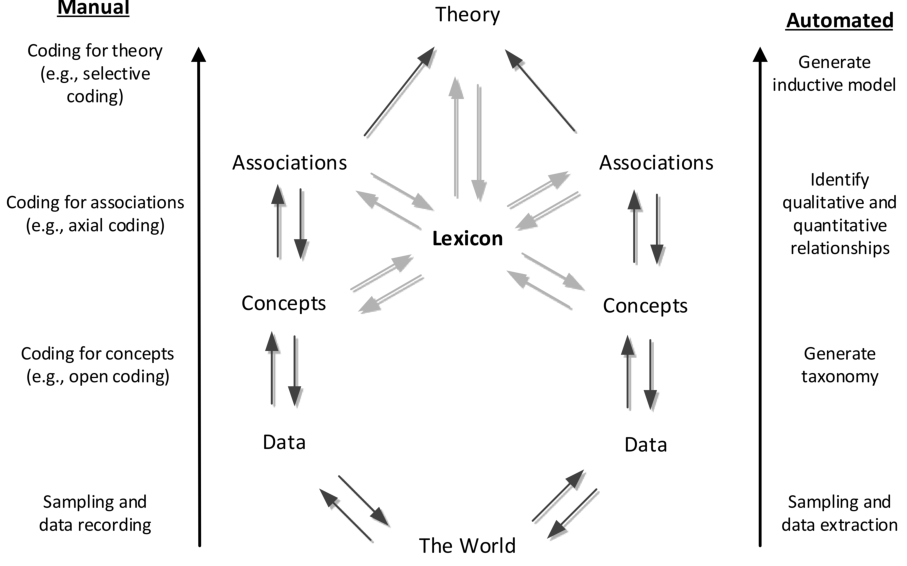
\includegraphics[width=0.7\linewidth]{figures/empirically-driven-theory-generation-1}
%	\caption{Empirically driven theory generation \citep{Berente2018}}
%	\label{fig:empirically-driven-theory-generation}
%\end{figure}


%\begin{description}
%	\item[Guideline 1 -- Design as an Artifact.] Design-science research must produce a viable artifact in the form of a construct, a model, a method, or an instantiation In my research, I use state-of-the-art techniques and develop new artifacts that allow to capture information from both structured and unstructured types of data. 
%	
%	\item[Guideline 2 -- Problem Relevance.] The objective of design-science research is to develop technology based solutions to important and relevant business problems. My research takes inspiration from real world needs which include human-centric safety-critical automated solutions in the railway domain.  
%	
%	\item[Guideline 3 -- Design Evaluation.] The utility, quality, and efficacy of a design artifact must be rigorously demonstrated via well-executed evaluation methods. The real world scenarios that I encounter in the SHAPE project require for novel solutions, which involve the design of new algorithms. Algorithms are converted to operational software. This operational software is an instantiated artifact \citep{Gregor2013}, which is then tested against real data. 
%	
%	\item[Guideline 4 -- Research Contributions.] Effective design-science research must provide clear and verifiable contributions in the areas of the design artifact, design foundations, and/or design methodologies. The contribution of my research can be positioned as a set of \emph{exapted} methods (cf. \gls{dsr} knowledge contribution framework \citep{Gregor2013}) from the fields of process mining and text mining, which contribute to a better understanding of projects. 
%	
%	\item[Guideline 5 -- Research Rigor.] Design-science research relies upon the application of rigorous methods in both the construction and evaluation of the design artifact. My research builds upon existing work from natural language processing \citep{de2006generating,Corro2013,klein2003accurate}, a number of \gls{vcs} mining works \citep{Banitaan2015,Allamanis2013,Vasilescu2015,Karimi2016,German2015}, and process mining.
%%	\cite[]{van2011process,rubin2007process,Rubin2014a,rubin2014agile}. 
%I plan to adopt mature methods from the mentioned works and construct my artifacts upon existing ones. 
%	
%	\item[Guideline 6 -- Design as a Search Process.] 
%	The search for an effective artifact requires utilizing available means to reach desired ends while satisfying laws in the problem environment. I plan to build my artifacts based on state-of-the-art methods and technology and follow both a rigorous process as the one described in \citep{Peffers2008} (cf. \cref{fig:DS-process}). Given the nature of my data, an exploratory phase may be required in the initial activity of this process. This may involve exploratory data analysis, as described in the data science process \citep[p.~41]{Schutt2013}
%	
%	\item[Guideline 7 -- Communication of Research.] Design-science research must be presented effectively both to technology-oriented as well as management-oriented audiences. I will use guidelines \citep{Gregor2013,Recker2015} in order to properly position my work. The main target will be \gls{bpm} conferences and journals. 
%	
%\end{description}


\section{Generated Datasets}
\label{sec:data-collection}

%\todo[inline]{Is this the best place for this section?}

This thesis includes the collection of and generation of datasets from real life software projects. These project data were collected both from industrial partners and from \gls{oss}. \Cref{tab:dataset} summarizes the available data. Logs from industrial partner are concerned with specific development activities (e.g., building railway interlocking-system software) and include a sufficient number of events that cover one software release. Logs from \gls{oss} were manually extracted by GitHub repositories. A tool has then been devised to parse these data and use them to populate a database. An original dataset is represented by Github pull requests. This dataset contains a list of manually annotated pull requests using the coding scheme by \cite[]{Majchrzak2016}. An additional output of this thesis will be the creation of a larger dataset using a machine learning approach that is able to automatically categorize pull requests in the classes given by \cite[]{Majchrzak2016}.

% Please add the following required packages to your document preamble:
% \usepackage{booktabs}
\begin{table}[]
\centering
\caption{Available datasets for this thesis}
\label{tab:dataset}
\begin{tabular}{@{}m{2.5cm}m{9cm}@{}}
\toprule
\textbf{Event Logs} & \textbf{Description} \\ \midrule
SHAPE & Industry \gls{vcs} from software development in the railway domain \\
Github & Logs from real world \gls{oss} development \\
Github pull requests & Manually annotated pull requests from one real life open source project \\
Jira & Log data from \gls{its} from industry partner \\
Asana & Generated dataset from project management tool of industrial partner \\
Kibana & Event traces from distributed process-agnostic enviroment used to handle communication among several processes \\ \bottomrule
\end{tabular}
\end{table}

%\subsection{Expected Outcome}
%
%In addition to an original dataset, this doctoral thesis is expected to produce outcomes that help the project manager analyze his software development processes. To this end new approaches in the form of artifacts \citep{Peffers2008} will be devised. These artifacts will serve as proofs-of-concept for the applicability of the research. In particular, the artifacts must address each of the four process aspects. Therefore, the outcome is categorized according to the research questions derived in \Cref{sec:problem-definition} as follows.
%
%\begin{itemize}	
%	\item \textbf{Artifact A1: Mining the Time Perspective (RQ1)}. Novel technique that allows for gaining transparency on the time perspective of software development work.	For instance, and artifact that explicits what are the durations of tasks and when are actual tasks executed.
%	
%	\item \textbf{Artifact A2: Mining the Case Perspective (RQ2)}. Novel technique that allows for gaining transparency on the case perspective of software development work. For instance, an artifact that explicits how the different cases are handled and whether there is any dependency of work that might influence the case execution. 
%	
%	\item \textbf{Artifact A3: Mining the Organizational Perspective (RQ3)}. Novel technique that allows for gaining transparency on the organizations aspect of software development work. For instance, an artifact that explicits which are the actual roles software developers are covering and which is the organizational network. 
%	
%	\item \textbf{Artifact A4: Mining the Control-Flow Perspective (RQ4)}. Novel technique that allows for gaining transparency on the control-flow perspective of software development work. For instance, an artifact that allows for abstracting from data which is order of activities that are executed to accomplish a certain task or goal in software development.	
%\end{itemize}

%\Cref{fig:big-solution} shows the overall information coming from combining the four perspectives into a Gantt chart that is more informative to managers. 




\section{Research Contributions}
\label{sec:intro-contributions}

%\todo[inline]{Summarize contributions beyond the papers. E.g., visualisation, conceptualisation of process-oriented business processes, etc. Elaborate more and think of further contributions.}

This doctoral thesis aims at bridging the gap between automatic analysis of software development data and process mining. It provides analyses techniques that help learning specific characteristics of the software process from its trace data. Beyond the publications, this thesis makes the following contributions.

\begin{itemize}
	
	\item \textbf{Conceptualization of project-oriented business processes.} Processes have been seen so far as repeatable endeavors. However, there are processes which are not repeated exactly in the same way twice. This is the case with project-oriented business processes. Such processes, are conducted as projects, in that they are usually planned a priori and run under limited resources. 
	
	\item \textbf{Visualization.} Existing techniques in the software engineering area are able to provide several possible views on the software development. Major visualization techniques can be divided into graph-based \citep{DBLP:journals/ijseke/GermanH06,DBLP:journals/smr/GreevyDG06}, notation-based \citep{DBLP:conf/wcre/McNairGW07}, matrix-based \citep{DBLP:conf/icsm/GirbaDL04} and metaphor-based \citep{DBLP:conf/vissoft/WettelL07}. These visualization techniques help in multiple ways, such as understanding code smells, refactoring, evolution, distribution of work etc. However, most of the works in software engineering area are not process-aware. Thus, this thesis aims at researching the most suitable visualization techniques that help understanding the work process that lays behind software development. 	

	\item \textbf{Extension of the scope of process mining.} Process mining techniques rely on structured data. These data are typically captured by the standard XES \citep{xes-standard:2015} which defines precisely the input of process mining techniques. This work extends process mining towards mining processes also from data that are not directly represented in the XES standard. 
	
	\item \textbf{Datasets for further research.} During the course of this research a number of datasets have been generated. These datasets are available for further use by researchers who want to replicate these studies or pursue different goals using the same concepts that this thesis provides. 
	
\end{itemize}



\section{Thesis Structure}
\label{sec:intro-structure}

%\todo[inline]{Elaborate more the description of what the sections provide.}

This thesis is structured as follows. 

\begin{itemize}
	\item \textbf{Chapter 1: Introduction} motivates research on the topic of mining processes from software repositories. This chapter also scopes the problem addressed by this dissertation and provides an overall guide to the content of this manuscript.
	
	\item \textbf{Chapter 2: Research Background} presents the body of knowledge which inform this thesis. 
%	\item \textbf{Chapter 3: Data-Driven Approaches to Analyzing the Software Process} 
	This chapter also elaborates on existing solutions and techniques that are present in the literature which are used as a base to develop new artifacts for mining the software process. 
	
	\item \textbf{Chapter 3: Discovering the Temporal Perspective} tackles the problem of discovering the temporal aspect (RQ1) of the software development process. A visualization technique is presented that simplifies the managers' understanding of such perspective.
	
	\item \textbf{Chapter 4: Discovering the Case Perspective}  presents an approach that helps understanding how different artifacts co-evolve in software development. With this approach, it is possible to compare how similarly different artifacts evolve and consequently cluster them into similar development cases (RQ2).  
	
	\item \textbf{Chapter 5: Discovering the Organizational Perspective} tackles the problem of automatically identifying emerging roles in software development. Thus, a technique for classifying human-resources (RQ3) based on factual data is presented.
	
	\item \textbf{Chapter 6: Discovering the Control-Flow Perspective} complements the techniques presented in previous chapter with the information about which activities were executed by resources. These activity labels along with the temporal help understanding the control-flow (RQ4) of the development process.
	
	\item \textbf{Chapter 7: Case Study in an Austrian Enterprise} presents an approach which uses a mixed-method to gather insights on the process. This approach aims at evaluating the existing status of the software development process by analysing the \gls{sdm} of the company. This is achieved by considering the constituting elements of the methodolody. In this approach, trace data analysis of software repositories is combined with subjective information from questionnaire. Mixing these methods helps to better identify issues in and suggest interventions based on facts. In this sense, this chapter provides a practical application of the concepts presented in this thesis on a real world company (RQ 1--4).
	
	\item \textbf{Chapter 8: Conclusion} summarizes the main findings. Further more, it discusses their implications along with future research. 
	 	
\end{itemize}


\section{Publications}
\label{sec:intro-related-publications}

This dissertation has led to the publications listed below.\\

\noindent {Mining the Time Perspective(\textbf{RQ1}):}~\citep{DBLP:conf/bpm/BalaCMRP15}
\begin{itemize}
\item \textbf{Bala, S.}, Cabanillas, C., Mendling, J., Rogge-Solti, A., and Polleres, A.: \textit{Mining Project-Oriented Business Processes}. In Hamid Reza Motahari-Nezhad, Jan Recker, and Matthias Weidlich, editors, BPM 2015, Innsbruck, Austria, volume 9253 of Lecture Notes in Computer Science, pages 425--440. Springer, 2015. 
\end{itemize}	
\noindent {Mining the Case Perspective (\textbf{RQ2}):}~\citep{DBLP:conf/bpm/BalaRGBMS17}.
\begin{itemize}
	\item \textbf{Bala, S.}, Revoredo, K., de A.R. Gonçalves, J.C., Baião, F., Mendling, J., Santoro, F.: \textit{Uncovering the Hidden Co-evolution in the Work History of Software Projects}. In: Carmona, J., Engels, G., and Kumar, A. (eds.) Business Process Management - 15th International Conference, BPM 2017, Barcelona, Spain, September 10-15, 2017, Proceedings. pp. 164--180. Springer (2017). 
\end{itemize}
\noindent {Mining the Organizational Perspective (\textbf{RQ3}):} \citep{DBLP:conf/edoc/AgrawalATBRT16}.
\begin{itemize}
	\item Agrawal, K., Aschauer, M., Thonhofer, T., \textbf{Bala, S.}, Rogge-Solti, A., Tomsich, N.: \textit{Resource Classification from Version Control System Logs}. In: Proceedings - IEEE International Enterprise Distributed Object Computing Workshop, EDOC Workshop. pp. 249--258 (2016). 
\end{itemize}
\noindent {Mining the Control-Flow Perspective (\textbf{RQ4}):} \citep{DBLP:conf/ifip8-1/BalaKM20}
\begin{itemize}
	\item \textbf{Bala, S.}, Kneringer, P., \& Mendling, J.: \textit{Discovering Activities in Software Development Processes}. In: CEUR Workshop Proceedings. (2020)
\end{itemize}

\noindent The following publications are related to the requirements.
\begin{itemize}
	
\item \textbf{Bala, S.}, Cabanillas, C., Haselböck, A., Havur, G., Mendling, J., Polleres, A., Sperl, S., Steyskal, S.: \textit{A Framework for Safety-Critical Process Management in Engineering Projects}. In: Ceravolo, P. and Rinderle-Ma, S. (eds.) Data-Driven Process Discovery and Analysis- SIMPDA. pp. 1--27. Springer (2015). \cite[]{Bala2017} -- Related to \textbf{RQ1} \& \textbf{RQ3}.
	
\item \textbf{Bala, S.}, Havur, G., Sperl, S., Steyskal, S., Haselböck, A., Mendling, J., Polleres, A.: \textit{SHAPEworks: A BPMS extension for complex process management}. In: CEUR Workshop Proceedings. pp. 50--55 (2016). \cite[]{Bala2016} -- Related to \textbf{RQ1} \& \textbf{RQ3}.
	
\end{itemize}

\noindent Early stage concepts of this research (research proposal) have been presented in doctoral consortium and conference.
\begin{itemize}
	\item \textbf{Bala, S.}: \textit{Mining projects from structured and unstructured data}. In: CEUR Workshop Proceedings (2017). \cite[]{Bala2017b}

	\item \textbf{Bala, S.}, Mendling, J.: \textit{Monitoring the Software Development Process
		with Process Mining}. In Boris Shishkov, editor, Business Modeling and Software
	Design, volume 319 of Lecture Notes in Business Information Processing, 2018 \citep{Bala2018b} 	
\end{itemize}	
	

\noindent Further work published in the \gls{bpm} area is the following.

\begin{itemize}
	\item Woli\'nski, B., \textbf{Bala, S.}: \textit{Comprehensive Business Process Management at Siemens: Implementing Business Process Excellence}. In: vom Brocke, J. and Mendling, J. (eds.) Business Process Management Cases: Digital Innovation and Business Transformation in Practice. pp. 111--124. Springer International Publishing, Cham (2018). \cite[]{Wolinski2018}
	
	\item \textbf{Bala, S.}, Mendling, J., Schimak, M. and Queteschiner, P., 2018, October. \textit{Case and activity identification for mining process models from middleware}. In IFIP Working Conference on The Practice of Enterprise Modeling (pp. 86-102). Springer, Cham. \citep{DBLP:conf/ifip8-1/BalaMSQ18}
	
	\item Azemi, E., \textbf{Bala, S.}: \textit{Exploring BPM adoption and strategic alignment of processes at Raiffeisen Bank Kosovo}. In: BPM (Industry Forum). pp. 37–48. CEUR-WS.org (2019). \cite[]{DBLP:conf/bpm/AzemiB19}
	
	\item Vidgof, M., Djurica, D., \textbf{Bala, S.}, and Mendling, J. (2020). \textit{Cherry-picking from
	spaghetti: Multi-range filtering of event logs}. In BPMDS/EMMSAD@CAiSE,
	volume 387 of Lecture Notes in Business Information Processing, pages 135–149.
	Springer. \citep{DBLP:conf/caise/VidgofDBM20}
	
	\item Vidgof, M., Djurica, D., \textbf{Bala, S.}, Mendling, J.: \textit{Interactive Log-Delta-Analysis using Multi-Range Filtering}. Software and Systems Modeling, (2021). \citep{Vidgof2021}
	
	\item Azemi, E., \textbf{Bala, S.}: \textit{Exploring BPM adoption and strategic alignment of processes at Raiffeisen Bank Kosovo}. In: vom Brocke, J., Mendling, J., Rosemann, M. (eds.) Business Process Management Cases. Springer (2021). \citep{Azemi2021}
	
	\item Waibel, P., Novak, C., \textbf{Bala, S.}, Revoredo, K., Mendling, J.: \textit{Analysis of Business Process Batching Using Causal Event Models}. In: Leemans, S.J.J. and Leopold, H. (eds.) ICPM Workshops. pp. 1–13. Springer Nature Switzerland AG (2021). \citep{Waibel2021}
	
\end{itemize}

%\noindent From ongoing work the following publications are expected.
%\begin{itemize}
%	\item Case study on tool productivity. Collaboration with researchers from the University of Ljubljana to be submitted to an A-ranked journal on information systems. -- Related to \textbf{RQ1}, \textbf{RQ3} and \textbf{RQ4}.
%	
%	\item Process mining pull requests for identifying idea-creation patterns. Collaboration with researchers from Stevens Institute of Technology to be submitted to a class A journal on information systems -- Related to \textbf{RQ4}.
%	
%	\item Wurm, B., \textbf{Bala, S.}, Kremser, W., Mendling, J., Minaar, R., Strauss, E.: Working title: \textit{How holacratic organizations use information technology to prevent inertia of organizational rule networks}.  to submitted to Information Systems Research 
%		
%\end{itemize}

